\documentclass[]{beamer}
%language
\usepackage[ngerman,english]{babel}
\usepackage[utf8]{inputenc}

%\usepackage[usenames,dvipsnames]{xcolor}

\usepackage{tikz}
\usetikzlibrary{mindmap}

\usepackage[utf8]{inputenc}
%theme
\useoutertheme[nofootline]{wuerzburg}
\useinnertheme{chamfered}
\usecolortheme{shark}

%title setup
\title{Generischer Titel: Studie - Emailkryptographie}
%\subtitle{Montag 12-14, Raum 01.150-128}
\subtitle{Human Factors in IT-Security}
\author{Ulrich Dorsch, Tim Grocki, Leonhard Hösch  \\ {\tiny ulrichdorsch@googlemail.com, tgrocki@lavabit.com, lh@dancingwolf.de \\}}
\institute[Universität Erlangen]{Friedrich-Alexander-Universität Erlangen
\\Department Informatik \\ Lehrstuhl 1}


\AtBeginSection[]
{
	\begin{frame}
		\frametitle{Inhalt}
		\tiny{\tableofcontents[currentsection]}
	\end{frame}
}

\definecolor{goldenrod}{HTML}{FFDF42}

\begin{document}

\begin{frame}[plain]
	\begin{center}
		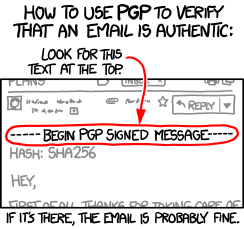
\includegraphics[scale=0.7]{pic/pgp.png}\phantom{\footnote{\url{http://xkcd.com/1181/}}}
	\end{center}
\end{frame}

%titlepage
\begin{frame}[plain]
	\titlepage
\end{frame}


\section{Zielsetzungen der Studie}

\subsection{Motivation}
\begin{frame}{Motivation}
\begin{itemize}
	\item Emailkryptographie ist nicht weit verbreitet, obwohl es viele Gründe für deren Einsatz gibt.
	\item Es wird of vermutet, dass schlechte Usability der Grund für die geringe Verbreitung ist.
	\item Wir haben dies mit unserer Studie überprüft.
\end{itemize}
\end{frame}


\subsection{Forschungsfrage}
\begin{frame}{Forschungsfrage}
	Sind Usability Probleme tatsächlich die Hauptgründe für die geringe Verbreitung von Emailkryptographie?

	\vspace{1.2cm}
	\onslide<2>{Welche anderen Ursachen spielen eine (wie große) Rolle?}
\end{frame}

\subsection{Hypothese}
\begin{frame}{Hypothese}
	Usability Probleme von Kryptographie-Software sind nicht die primäre Ursache für die geringe Verbreitung von Emailkryptographie, da mehr als 50\% der
	Nutzer von Emailkommunikation durch andere Ursachen davon abgehalten werden,
	Emailkryptographie einzusetzen.
	\onslide<2>{
		\begin{block}{Usability Problem - Definition}
			In unserem Kontext betrachten wir ein Usability Problem als eine technische Hürde,
			die die Benutzung von Emailkryptographie verhindert oder deutlich erschwert.
		\end{block}
	}
\end{frame}

\section{Umfrageumstände}
%% NSA
\begin{frame}{NSA Skandal}
	\begin{itemize}
	\item Der NSA-Skandal ging im Zeitraum unserer Umfrage durch alle Medien
		\footnote{\url{http://www.tagesschau.de/ausland/spionageaffaere100.html}}
	\item Überwachung des Internets, insbesondere von Emails
	\item Überwachung auch in Deutschland
	\item $\Rightarrow$ Erhöhtes Bewusstsein für IT-Sicherheit und die Existenz von
		Eingriffen in die Privatsphäre
	\end{itemize}
\end{frame}

\section{Demographische Daten}
\begin{frame}{Zielgruppe}
	Studenten (an der technischen Fakultät der Universität Erlangen)
\onslide<2>{
	\begin{itemize}
		\item einfach zu erreichen
		\item höchstwahrscheinlich aktive Nutzer von Emailkommunikation
		\item "zukünftige Elite Deutschlands"
		\item ca. 9000 Personen
	\end{itemize}
}
\end{frame}

\begin{frame}{Rücklauf}
	\begin{itemize}
		\item 207 vollständige und verwertbare Rückläufer
		\item ca. $2,3\%$ der vorhandenen Zielgruppe
		\item Rückläufer aus diversen Studienfächern
	\end{itemize}
\end{frame}

\begin{frame}{Demographische Daten}
	\begin{center}
		Studienfächer
	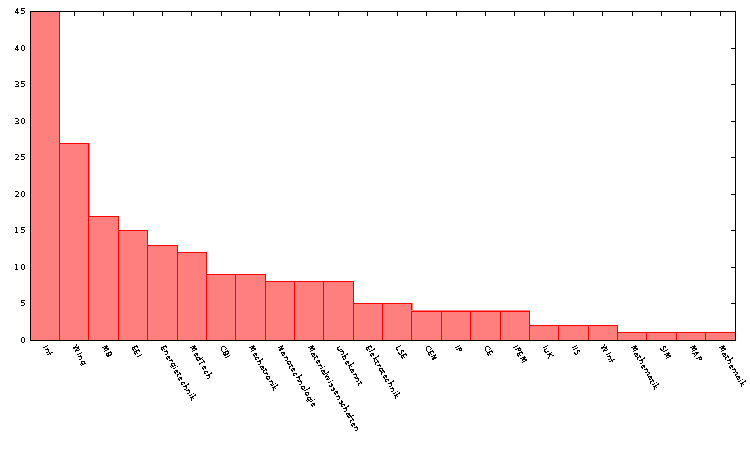
\includegraphics[scale=0.9]{plots/stud.pdf}
	\end{center}
\end{frame}

\section{Auswertung der Antworten}
\subsection{Interesse an Emailkryptographie}
\begin{frame}{Interesse an Emailkryptographie}
	\begin{center}
		\only<1>{Halten Sie das Verschlüsseln von Emails für sich persönlich für sinnvoll?\\
			\vspace{1cm}
				Ja: 51\% Nein: 41\% N/A: 08\%
		}
		\only<2>{Halten Sie das Verschlüsseln von Email im Allgemeinen für sinnvoll?\\
			\vspace{1cm}
				Ja: 87\% Nein: 06\% N/A: 07\%
		}
		\only<3>{Hätten Sie gerne die Möglichkeit mit Banken oder ähnlichen Institutionen/Firmen verschlüsselt zu kommunizieren?\\
			\vspace{1cm}
				Ja: 83\% Nein: 07\% N/A: 11\%
		}
		\only<4>{Würden Sie sich wünschen, dass Firmen wie Banken intern verschlüsselt kommunizieren?\\
			\vspace{1cm}
				Ja: 85\% Nein: 06\% N/A: 09\%
		}
	\end{center}
\end{frame}

\subsection{Bekanntheit von Gefahren}
\begin{frame}{Bekanntheit von Gefahren}
	  \begin{center}
		  \only<1>{ Eine unverschlüsselte Email, die Sie versenden, kann auf dem Zustellweg von einem Angreifer mitgelesen und verändert werden. \\ Wussten Sie das?\\
			  \vspace{1cm}
      Ja: 82\% Nein: 15\% N/A: 02\%
  }
  \only<2>{ Emails können mit sehr geringem Aufwand unter falschem Absender versendet werden, wenn diese nicht kryptographisch signiert sind. \\ Wussten Sie das?\\
	  \vspace{1cm}
      Ja: 68\% Nein: 29\% N/A: 03\%
  }
  \only<3>{ Sollte ein Angreifer (Hacker) administrative Zugriffsrechte auf den Server einer Firma erlangen kann dieser alle unverschlüsselten Emails der Firma lesen oder sogar verändern. \\ Wussten Sie das?\\
	  \vspace{1cm}
      Ja: 84\% Nein: 14\% N/A: 03\%
  }
  \end{center}	
\end{frame}


%%%% 'Emailkryptographie' unbekannt
\subsection{Schema des Fragebogens}

\begin{frame}{Fragebogenverlauf}
	Der Rest des Fragebogens ist baumartig strukturiert, sodass eine Einteilung
	in verschiedene Kategorien (diverse Ursachen für geringe Verbreitung von
	Emailkryptographie) leichtfällt.

	TODO: Legende für folgenden Baum, evtl weitere Erklärung
\end{frame}

\begin{frame}{Fragebogenverlauf}
	\begin{tikzpicture}[mindmap,scale=0.7]
		\path[concept color=goldenrod,every concept/.append style={scale=0.7}]
		node[concept] {{\huge $207$ \\ $100\%$}}
			child[concept color=blue,grow=-5] {node[concept,scale=1.3] {$65$ \\ $31.40\%$}}
			child[concept color=gray,grow=-170] {node[concept] {}
				child[concept color=gray,grow=-30] {node[concept] {}
					child[concept color=gray,grow=-90] {node[concept] {}
						child[concept color=gray,grow=-130] {node[concept] {}}
						child[concept color=gray,grow=-70] {node[concept] {}}
					}
					child[concept color=gray,grow=-10] {node[concept] {}
						child[concept color=gray,grow=0] {node[concept] {}}
						child[concept color=gray,grow=-60] {node[concept] {}
							child[concept color=gray,grow=-130] {node[concept] {}}
							child[concept color=gray,grow=-50] {node[concept] {}}
						}
					}
				}
				child[concept color=gray,grow=-130] {node[concept] {}
					child[concept color=gray,grow=-130] {node[concept] {}}
					child[concept color=gray,grow=-70] {node[concept] {}
						child[concept color=gray,grow=-130] {node[concept] {}}
						child[concept color=gray,grow=-70] {node[concept] {}
							child[concept color=gray,grow=-130] {node[concept] {}}
							child[concept color=gray,grow=-70] {node[concept] {}}
						}
					}
				}
			};
			\node[annotation,below,fill=gray!50,scale=1.3] at (4,-6.4) {Der Begriff "Emailkryptographie" ist unbekannt.};
	\end{tikzpicture}
\end{frame}

\begin{frame}{Details}
	\begin{center}
	Studenten, die den Begriff "Emailkryptographie" nicht kennen:
	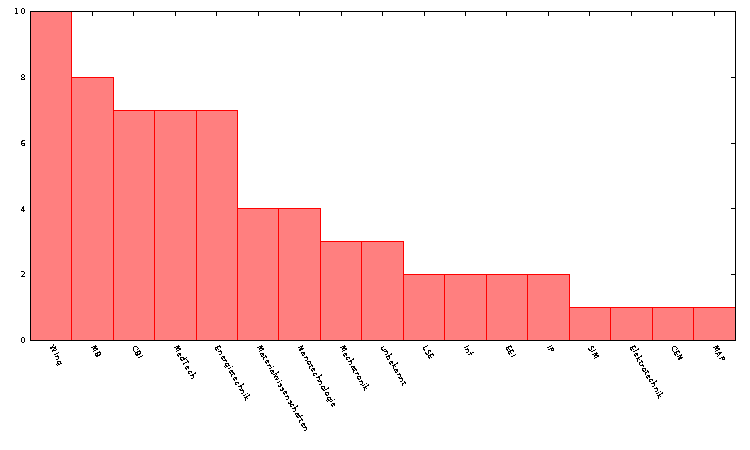
\includegraphics[scale=0.9]{plots/emailkryptunbek.pdf}
\end{center}
\end{frame}
\begin{frame}{Details}
	$65$ Studenten, die den Begriff "Emailkryptographie" nicht kennen:
	\begin{itemize}
		\item Die Studenten sind im Durchschnitt im $5.1$-ten Semester\\ (Standardabw.: $2.9$, Maximum: $12$)
		\item<2-> OS: $53$ nutzen Microsoft Windows, $9$ nutzen Mac OS
		\item<3-> Emailclients: $37$ nutzen Seamonkey, $11$ OS X Mail, $8$ Thunderbird, häufig zusätzliche Nutzung von Webclients, Smartphones
	\end{itemize}
\end{frame}

%%%% Emailkryptographie regelmäßig eingesetzt
\begin{frame}{Fragebogenverlauf}
	\begin{tikzpicture}[mindmap,scale=0.7]
		\path[concept color=goldenrod,every concept/.append style={scale=0.7}]
		node[concept] {$207$ \\ $100\%$}
			child[concept color=gray,grow=-5] {node[concept] {$65$ \\ $31.40\%$}}
			child[concept color=goldenrod,grow=-170] {node[concept] {$142$ \\ $68,60\%$}
				child[concept color=gray,grow=-30] {node[concept] {}
					child[concept color=gray,grow=-90] {node[concept] {}
						child[concept color=gray,grow=-130] {node[concept] {}}
						child[concept color=gray,grow=-70] {node[concept] {}}
					}
					child[concept color=gray,grow=-10] {node[concept] {}
						child[concept color=gray,grow=0] {node[concept] {}}
						child[concept color=gray,grow=-60] {node[concept] {}
							child[concept color=gray,grow=-130] {node[concept] {}}
							child[concept color=gray,grow=-50] {node[concept] {}}
						}
					}
				}
				child[concept color=goldenrod,grow=-130] {node[concept] {$54$ \\ $26.09\%$}
					child[concept color=blue,grow=-130] {node[concept] {$30$ \\ $14.49\%$}}
					child[concept color=gray,grow=-70] {node[concept] {}
						child[concept color=gray,grow=-130] {node[concept] {}}
						child[concept color=gray,grow=-70] {node[concept] {}
							child[concept color=gray,grow=-130] {node[concept] {}}
							child[concept color=gray,grow=-70] {node[concept] {}}
						}
					}
				}
			};
			\node[annotation,below,fill=gray!50,scale=1.3] at (4,-6.4) {Emailkryptographie wird regelmäßig eingesetzt.};
	\end{tikzpicture}
\end{frame}

\begin{frame}{Details}
	Studenten, die Emailkryptographie regelmäßig einsetzen:
  \begin{itemize}
	\item $30$ Studenten, davon $18$ Informatiker
	\item<2-> $29$ finden, dass ihre Software einfach zu bedienen ist
	\item<2-> $1$ Informatiker ($12.$ Semester, Emailclient: Thunderbird, OS: Linux) findet seine Software schwer zu bedienen
	\item<3-> Die Studenten verschicken im Durchschnitte $8.5$ verschlüsselte Mails im Monat (Standardabw.: $8.3$, Maximum: $30$)
	\item<4-> Die Studenten haben im Durchschnitt $4.1$ Kontakte, mit denen sie verschlüsselt kommuniziert können
		(Standardabw.: $5.2$, Maximum: $25$)
	\item<5-> $17$ Studenten nutzen Thunderbird, $8$ OS X Mail, oft in Kombination mit Webclient und Smartphone
  \end{itemize}
\end{frame}


%%%% min 1x eingesetzt

\begin{frame}{Fragebogenverlauf}
	\begin{tikzpicture}[mindmap,scale=0.7]
		\path[concept color=goldenrod,every concept/.append style={scale=0.7}]
		node[concept] {$207$ \\ $100\%$}
			child[concept color=gray,grow=-5] {node[concept] {$65$ \\ $31.40\%$}}
			child[concept color=goldenrod,grow=-170] {node[concept] {$142$ \\ $68,60\%$}
				child[concept color=gray,grow=-30] {node[concept] {}
					child[concept color=gray,grow=-90] {node[concept] {}
						child[concept color=gray,grow=-130] {node[concept] {}}
						child[concept color=gray,grow=-70] {node[concept] {}}
					}
					child[concept color=gray,grow=-10] {node[concept] {}
						child[concept color=gray,grow=0] {node[concept] {}}
						child[concept color=gray,grow=-60] {node[concept] {}
							child[concept color=gray,grow=-130] {node[concept] {}}
							child[concept color=gray,grow=-50] {node[concept] {}}
						}
					}
				}
				child[concept color=goldenrod,grow=-130] {node[concept] {$54$ \\ $26.09\%$}
					child[concept color=gray,grow=-130] {node[concept] {$30$ \\ $14.49\%$}}
					child[concept color=goldenrod,grow=-70] {node[concept] {$24$ \\ $11.59\%$}
						child[concept color=violet,grow=-130] {node[concept] {$17$ \\ $8.21\%$}}
						child[concept color=gray,grow=-70] {node[concept] {}
							child[concept color=gray,grow=-130] {node[concept] {}}
							child[concept color=gray,grow=-70] {node[concept] {}}
						}
					}
				}
			};
			\node[annotation,below,fill=gray!50,scale=1.3] at (4,-6.4) {Emailkryptographie wurde schon mindestens einmal eingesetzt.};
	\end{tikzpicture}
\end{frame}
\begin{frame}{Details}
  \begin{itemize}
    \item Keine meiner Kommunikationspartner hält es für nötig und da zu Verschlüsselung immer zwei gehören, erübrigt sich das ganze Vorhaben.
    \item Weil ich die Erfahrung gemacht habe, dass der Empfänger, selbst wenn er einen PGP-Key besitzt und veröffentlicht hat,  diese meist nicht entschlüsseln kann, weil er die passende Softwware nicht installiert hat. Meistens ist es wichtiger, dass eine E-Mail ankommt, als dass sie verschlüsselt ist.
    \item Android-Handy (und GMail Webinterface) unterstützen keine verschlüsselten Mails, insbesondere empfangene, verschlüsselte Mails könnten nicht einmal gelesen werden.
    \item Im Umfeld außerhalb des Arbeitsplatzes nicht sehr verbreitet.
Per Email werden daher auch keine wichtigen Informationen versendet.
  \end{itemize}
\end{frame}


%%%% noch nie eingesetzt trotz vorhandener kontakte
\begin{frame}{Fragebogenverlauf}
	\begin{tikzpicture}[mindmap,scale=0.7]
		\path[concept color=goldenrod,every concept/.append style={scale=0.7}]
		node[concept] {$207$ \\ $100\%$}
			child[concept color=gray,grow=-5] {node[concept] {$65$ \\ $31.40\%$}}
			child[concept color=goldenrod,grow=-170] {node[concept] {$142$ \\ $68,60\%$}
				child[concept color=gray,grow=-30] {node[concept] {}
					child[concept color=gray,grow=-90] {node[concept] {}
						child[concept color=gray,grow=-130] {node[concept] {}}
						child[concept color=gray,grow=-70] {node[concept] {}}
					}
					child[concept color=gray,grow=-10] {node[concept] {}
						child[concept color=gray,grow=0] {node[concept] {}}
						child[concept color=gray,grow=-60] {node[concept] {}
							child[concept color=gray,grow=-130] {node[concept] {}}
							child[concept color=gray,grow=-50] {node[concept] {}}
						}
					}
				}
				child[concept color=goldenrod,grow=-130] {node[concept] {$54$ \\ $26.09\%$}
					child[concept color=gray,grow=-130] {node[concept] {$30$ \\ $14.49\%$}}
					child[concept color=goldenrod,grow=-70] {node[concept] {$24$ \\ $11.59\%$}
						child[concept color=gray,grow=-130] {node[concept] {$17$ \\ $8.21\%$}}
						child[concept color=goldenrod,grow=-70] {node[concept] {$7$ \\ $3.38\%$}
							child[concept color=red,grow=-130] {node[concept] {$6$ \\ $2.90\%$}}
							child[concept color=gray,grow=-70] {node[concept] {}}
						}
					}
				}
			};
			\node[annotation,below,fill=gray!50,scale=1.3] at (4,-6.4) {Emailkryptographie wurde noch nie eingesetzt, obwohl Kontakte vorhanden wären, mit denen
			verschlüsselte Kommunikation möglich wäre.};
	\end{tikzpicture}
\end{frame}

\begin{frame}{Details}
	TODO
\end{frame}

%%%% keine kontakte vorhanden
\begin{frame}{Fragebogenverlauf}
	\begin{tikzpicture}[mindmap,scale=0.7]
		\path[concept color=goldenrod,every concept/.append style={scale=0.7}]
		node[concept] {$207$ \\ $100\%$}
			child[concept color=gray,grow=-5] {node[concept] {$65$ \\ $31.40\%$}}
			child[concept color=goldenrod,grow=-170] {node[concept] {$142$ \\ $68,60\%$}
				child[concept color=gray,grow=-30] {node[concept] {}
					child[concept color=gray,grow=-90] {node[concept] {}
						child[concept color=gray,grow=-130] {node[concept] {}}
						child[concept color=gray,grow=-70] {node[concept] {}}
					}
					child[concept color=gray,grow=-10] {node[concept] {}
						child[concept color=gray,grow=0] {node[concept] {}}
						child[concept color=gray,grow=-60] {node[concept] {}
							child[concept color=gray,grow=-130] {node[concept] {}}
							child[concept color=gray,grow=-50] {node[concept] {}}
						}
					}
				}
				child[concept color=goldenrod,grow=-130] {node[concept] {$54$ \\ $26.09\%$}
					child[concept color=gray,grow=-130] {node[concept] {$30$ \\ $14.49\%$}}
					child[concept color=goldenrod,grow=-70] {node[concept] {$24$ \\ $11.59\%$}
						child[concept color=gray,grow=-130] {node[concept] {$17$ \\ $8.21\%$}}
						child[concept color=goldenrod,grow=-70] {node[concept] {$7$ \\ $3.38\%$}
							child[concept color=gray,grow=-130] {node[concept] {$6$ \\ $2.90\%$}}
							child[concept color=blue,grow=-70] {node[concept] {$1$ \\ $0.48\%$}}
						}
					}
				}
			};
			\node[annotation,below,fill=gray!50,scale=1.3] at (4,-6.4) {Keine Kontakte, mit denen verschlüsselte Kommunikation möglich ist, vorhanden.};
	\end{tikzpicture}
\end{frame}

\begin{frame}{Details}
	TODO
\end{frame}

%%%% schonmal installiert, bewusst entfernt
\begin{frame}{Fragebogenverlauf}
	\begin{tikzpicture}[mindmap,scale=0.7]
		\path[concept color=goldenrod,every concept/.append style={scale=0.7}]
		node[concept] {$207$ \\ $100\%$}
			child[concept color=gray,grow=-5] {node[concept] {$65$ \\ $31.40\%$}}
			child[concept color=goldenrod,grow=-170] {node[concept] {$142$ \\ $68,60\%$}
				child[concept color=goldenrod,grow=-30] {node[concept] {$88$ \\ $42.51\%$}
					child[concept color=goldenrod,grow=-90] {node[concept] {$15$ \\ $7.25\%$}
						child[concept color=red,grow=-130] {node[concept] {$9$ \\ $4.35\%$}}
						child[concept color=gray,grow=-70] {node[concept] {}}
					}
					child[concept color=gray,grow=-10] {node[concept] {}
						child[concept color=gray,grow=0] {node[concept] {}}
						child[concept color=gray,grow=-60] {node[concept] {}
							child[concept color=gray,grow=-130] {node[concept] {}}
							child[concept color=gray,grow=-50] {node[concept] {}}
						}
					}
				}
				child[concept color=gray,grow=-130] {node[concept] {$54$ \\ $26.09\%$}
					child[concept color=gray,grow=-130] {node[concept] {$30$ \\ $14.49\%$}}
					child[concept color=gray,grow=-70] {node[concept] {$24$ \\ $11.59\%$}
						child[concept color=gray,grow=-130] {node[concept] {$17$ \\ $8.21\%$}}
						child[concept color=gray,grow=-70] {node[concept] {$7$ \\ $3.38\%$}
							child[concept color=gray,grow=-130] {node[concept] {$6$ \\ $2.90\%$}}
							child[concept color=gray,grow=-70] {node[concept] {$1$ \\ $0.48\%$}}
						}
					}
				}
			};
			\node[annotation,below,fill=gray!50,scale=1.3] at (4,-6.4) {Software für Emailkryptographie war schonmal installiert, wurde jedoch bewusst wieder entfernt.};
	\end{tikzpicture}
\end{frame}

\begin{frame}{Details}
	TODO
\end{frame}

%%%% schonmal installiert, unbewusst entfernt
\begin{frame}{Fragebogenverlauf}
	\begin{tikzpicture}[mindmap,scale=0.7]
		\path[concept color=goldenrod,every concept/.append style={scale=0.7}]
		node[concept] {$207$ \\ $100\%$}
			child[concept color=gray,grow=-5] {node[concept] {$65$ \\ $31.40\%$}}
			child[concept color=goldenrod,grow=-170] {node[concept] {$142$ \\ $68,60\%$}
				child[concept color=goldenrod,grow=-30] {node[concept] {$88$ \\ $42.51\%$}
					child[concept color=goldenrod,grow=-90] {node[concept] {$15$ \\ $7.25\%$}
						child[concept color=gray,grow=-130] {node[concept] {$9$ \\ $4.35\%$}}
						child[concept color=red,grow=-70] {node[concept] {$6$ \\ $2.90\%$}}
					}
					child[concept color=gray,grow=-10] {node[concept] {}
						child[concept color=gray,grow=0] {node[concept] {}}
						child[concept color=gray,grow=-60] {node[concept] {}
							child[concept color=gray,grow=-130] {node[concept] {}}
							child[concept color=gray,grow=-50] {node[concept] {}}
						}
					}
				}
				child[concept color=gray,grow=-130] {node[concept] {$54$ \\ $26.09\%$}
					child[concept color=gray,grow=-130] {node[concept] {$30$ \\ $14.49\%$}}
					child[concept color=gray,grow=-70] {node[concept] {$24$ \\ $11.59\%$}
						child[concept color=gray,grow=-130] {node[concept] {$17$ \\ $8.21\%$}}
						child[concept color=gray,grow=-70] {node[concept] {$7$ \\ $3.38\%$}
							child[concept color=gray,grow=-130] {node[concept] {$6$ \\ $2.90\%$}}
							child[concept color=gray,grow=-70] {node[concept] {$1$ \\ $0.48\%$}}
						}
					}
				}
			};
			\node[annotation,below,fill=gray!50,scale=1.3] at (4,-6.4) {Software für Emailkryptographie war schonmal installiert.};
	\end{tikzpicture}
\end{frame}

\begin{frame}{Details}
	TODO
\end{frame}

%%%% schonmal versucht zu installieren // gescheitert
\begin{frame}{Fragebogenverlauf}
	\begin{tikzpicture}[mindmap,scale=0.7]
		\path[concept color=goldenrod,every concept/.append style={scale=0.7}]
		node[concept] {$207$ \\ $100\%$}
			child[concept color=gray,grow=-5] {node[concept] {$65$ \\ $31.40\%$}}
			child[concept color=goldenrod,grow=-170] {node[concept] {$142$ \\ $68,60\%$}
				child[concept color=goldenrod,grow=-30] {node[concept] {$88$ \\ $42.51\%$}
					child[concept color=gray,grow=-90] {node[concept] {$15$ \\ $7.25\%$}
						child[concept color=gray,grow=-130] {node[concept] {$9$ \\ $4.35\%$}}
						child[concept color=gray,grow=-70] {node[concept] {$6$ \\ $2.90\%$}}
					}
					child[concept color=goldenrod,grow=-10] {node[concept] {$73$ \\ $35.27\%$}
						child[concept color=gray,grow=0] {node[concept] { }}
						child[concept color=goldenrod,grow=-60] {node[concept] {$19$ \\ $9.18\%$}
							child[concept color=red,grow=-130] {node[concept] {$1$ \\ $0.48\%$ }}
							child[concept color=gray,grow=-50] {node[concept] {}}
						}
					}
				}
				child[concept color=gray,grow=-130] {node[concept] {$54$ \\ $26.09\%$}
					child[concept color=gray,grow=-130] {node[concept] {$30$ \\ $14.49\%$}}
					child[concept color=gray,grow=-70] {node[concept] {$24$ \\ $11.59\%$}
						child[concept color=gray,grow=-130] {node[concept] {$17$ \\ $8.21\%$}}
						child[concept color=gray,grow=-70] {node[concept] {$7$ \\ $3.38\%$}
							child[concept color=gray,grow=-130] {node[concept] {$6$ \\ $2.90\%$}}
							child[concept color=gray,grow=-70] {node[concept] {$1$ \\ $0.48\%$}}
						}
					}
				}
			};
			\node[annotation,below,fill=gray!50,scale=1.3] at (4,-6.4) {Software für Emailkryptographie war noch nie installiert; es wurde schonmal versucht
			eine solche Software zu installieren (gescheitert).};
	\end{tikzpicture}
\end{frame}

\begin{frame}{Details}
	TODO
\end{frame}

%%%% installation geplant aber nie versucht
\begin{frame}{Fragebogenverlauf}
	\begin{tikzpicture}[mindmap,scale=0.7]
		\path[concept color=goldenrod,every concept/.append style={scale=0.7}]
		node[concept] {$207$ \\ $100\%$}
			child[concept color=gray,grow=-5] {node[concept] {$65$ \\ $31.40\%$}}
			child[concept color=goldenrod,grow=-170] {node[concept] {$142$ \\ $68,60\%$}
				child[concept color=goldenrod,grow=-30] {node[concept] {$88$ \\ $42.51\%$}
					child[concept color=gray,grow=-90] {node[concept] {$15$ \\ $7.25\%$}
						child[concept color=gray,grow=-130] {node[concept] {$9$ \\ $4.35\%$}}
						child[concept color=gray,grow=-70] {node[concept] {$6$ \\ $2.90\%$}}
					}
					child[concept color=goldenrod,grow=-10] {node[concept] {$73$ \\ $35.27\%$}
						child[concept color=gray,grow=0] {node[concept] {}}
						child[concept color=goldenrod,grow=-60] {node[concept] {$19$ \\ $9.18\%$}
							child[concept color=gray,grow=-130] {node[concept] {$1$ \\ $0.48\%$}}
							child[concept color=blue,grow=-50] {node[concept] {$18$ \\ $8.70\%$}}
						}
					}
				}
				child[concept color=gray,grow=-130] {node[concept] {$54$ \\ $26.09\%$}
					child[concept color=gray,grow=-130] {node[concept] {$30$ \\ $14.49\%$}}
					child[concept color=gray,grow=-70] {node[concept] {$24$ \\ $11.59\%$}
						child[concept color=gray,grow=-130] {node[concept] {$17$ \\ $8.21\%$}}
						child[concept color=gray,grow=-70] {node[concept] {$7$ \\ $3.38\%$}
							child[concept color=gray,grow=-130] {node[concept] {$6$ \\ $2.90\%$}}
							child[concept color=gray,grow=-70] {node[concept] {$1$ \\ $0.48\%$}}
						}
					}
				}
			};
			\node[annotation,below,fill=gray!50,scale=1.3] at (4,-6.4) {Software für Emailkryptographie war noch nie installiert; Installation war geplant, jedoch nie
			tatsächlich versucht.};
	\end{tikzpicture}
\end{frame}

\begin{frame}{Details}
	TODO
\end{frame}

%%%% installation nie geplant, nie versucht
\begin{frame}{Fragebogenverlauf}
	\begin{tikzpicture}[mindmap,scale=0.7]
		\path[concept color=goldenrod,every concept/.append style={scale=0.7}]
		node[concept] {$207$ \\ $100\%$}
			child[concept color=gray,grow=-5] {node[concept] {$65$ \\ $31.40\%$}}
			child[concept color=goldenrod,grow=-170] {node[concept] {$142$ \\ $68,60\%$}
				child[concept color=goldenrod,grow=-30] {node[concept] {$88$ \\ $42.51\%$}
					child[concept color=gray,grow=-90] {node[concept] {$15$ \\ $7.25\%$}
						child[concept color=gray,grow=-130] {node[concept] {$9$ \\ $4.35\%$}}
						child[concept color=gray,grow=-70] {node[concept] {$6$ \\ $2.90\%$}}
					}
					child[concept color=goldenrod,grow=-10] {node[concept] {$73$ \\ $35.27\%$}
						child[concept color=blue,grow=0] {node[concept] {$54$ \\ $26.09\%$}}
						child[concept color=gray,grow=-60] {node[concept] {$19$ \\ $9.18\%$}
							child[concept color=gray,grow=-130] {node[concept] {$1$ \\ $0.48\%$}}
							child[concept color=gray,grow=-50] {node[concept] {$18$ \\ $8.70\%$}}
						}
					}
				}
				child[concept color=gray,grow=-130] {node[concept] {$54$ \\ $26.09\%$}
					child[concept color=gray,grow=-130] {node[concept] {$30$ \\ $14.49\%$}}
					child[concept color=gray,grow=-70] {node[concept] {$24$ \\ $11.59\%$}
						child[concept color=gray,grow=-130] {node[concept] {$17$ \\ $8.21\%$}}
						child[concept color=gray,grow=-70] {node[concept] {$7$ \\ $3.38\%$}
							child[concept color=gray,grow=-130] {node[concept] {$6$ \\ $2.90\%$}}
							child[concept color=gray,grow=-70] {node[concept] {$1$ \\ $0.48\%$}}
						}
					}
				}
			};
			\node[annotation,below,fill=gray!50,scale=1.3] at (4,-6.4) {Software für Emailkryptographie war noch nie installiert; Installation war nie geplant.};
	\end{tikzpicture}
\end{frame}

\begin{frame}{Details}
	TODO
\end{frame}

\section{Forschungsergebnis}
\begin{frame}{Forschungsergebnis}
\begin{itemize}
	\item Von $207$ befragten setzen $30$ Emailkryptographie regelmäßig ein
	\item Von den restlichen $177$ werden (konservativ betrachtet) $39$ durch Usability Probleme
		vom Einsatz von Emailkryptographie abgehalten; dies entspricht $22.03\%$ der Befragten
	\item $77.97\%$ der Befragten werden also aus anderen Gründen vom Einsatz von Emailkryptographie abgehalten
	\item<2> die Hypothese ist somit bestätigt
\end{itemize}
	\only<2>{
		\begin{block}{Hypothese}
			Usability Probleme von Kryptographie-Software sind nicht die primäre Ursache für die geringe Verbreitung von Emailkryptographie, da mehr als 50\% der
	Nutzer von Emailkommunikation durch andere Ursachen davon abgehalten werden,
	Emailkryptographie einzusetzen.
		\end{block}
	}
	\only<3>{
		\begin{block}{andere Probleme}
			Unwissen\\
			Desinteresse\\
			mangelnde Motivation\\
			mangelnde Verbreitung von Emailkryptographie
		\end{block}
	}
\end{frame}

\section{Einschränkungen}
% meta probleme
% problem: knappe frage Emailkryptographie <-> unbekanter begriff
% hauptsächlich techniker/studenten
\begin{frame}{Einschränkungen}
	  \begin{itemize}
    \item indirekte Effekte schlechter Usability werden nicht betrachtet
    \item Frage nach dem Begriff "Emailkryptographie" problematisch
    \item nur Studenten aus technischen Fächern befragt
    \item technische Probleme
	\end{itemize}
\end{frame}

\section{Diskussion}
\begin{frame}{TODO}
	% witziges zeug, oder folgestudien
	TODO: evtl. abschließende Folie, was kann man mit weiteren Studien, wie und mit welchen Zielgruppen noch genauer untersuchen
\end{frame}

\begin{frame}{Diskussion}
  \begin{center}
	Fragen?

	Anmerkungen?
    
	Kritik?
    
	Diskussion!
	\end{center}
\end{frame}
\end{document}
